\documentclass{article}
\usepackage{amsmath,amssymb,mathtools}
\usepackage{xcolor}
\usepackage{minted}
\usepackage{enumitem}
\usepackage{multicol}
\usepackage{changepage}
\usepackage{stmaryrd}
\usepackage{graphicx}
\graphicspath{ {./images/} }
\usepackage[framemethod=tikz]{mdframed}
\usepackage{tikz,pgfplots}
\pgfplotsset{compat=1.18}

% physique
\definecolor{oranges}{RGB}{255, 242, 230}
\definecolor{rouges}{RGB}{255, 230, 230}
\definecolor{rose}{RGB}{255, 204, 204}

% maths - info
\definecolor{rouge_fonce}{RGB}{204, 0, 0}
\definecolor{rouge}{RGB}{255, 0, 0}
\definecolor{bleu_fonce}{RGB}{0, 0, 255}
\definecolor{vert_fonce}{RGB}{0, 69, 33}
\definecolor{vert}{RGB}{0,255,0}

\definecolor{orange_foncee}{RGB}{255, 153, 0}
\definecolor{myrtille}{RGB}{225, 225, 255}
\definecolor{mayonnaise}{RGB}{255, 253, 233}
\definecolor{magenta}{RGB}{224, 209, 240}
\definecolor{pomme}{RGB}{204, 255, 204}
\definecolor{mauve}{RGB}{255, 230, 255}


% Cours

\newmdenv[
  nobreak=true,
  topline=true,
  bottomline=true,
  rightline=true,
  leftline=true,
  linewidth=0.5pt,
  linecolor=black,
  backgroundcolor=mayonnaise,
  innerleftmargin=10pt,
  innerrightmargin=10pt,
  innertopmargin=5pt,
  innerbottommargin=5pt,
  skipabove=\topsep,
  skipbelow=\topsep,
]{boite_definition}

\newmdenv[
  nobreak=false,
  topline=true,
  bottomline=true,
  rightline=true,
  leftline=true,
  linewidth=0.5pt,
  linecolor=white,
  backgroundcolor=white,
  innerleftmargin=10pt,
  innerrightmargin=10pt,
  innertopmargin=5pt,
  innerbottommargin=5pt,
  skipabove=\topsep,
  skipbelow=\topsep,
]{boite_exemple}

\newmdenv[
  nobreak=true,
  topline=true,
  bottomline=true,
  rightline=true,
  leftline=true,
  linewidth=0.5pt,
  linecolor=black,
  backgroundcolor=magenta,
  innerleftmargin=10pt,
  innerrightmargin=10pt,
  innertopmargin=5pt,
  innerbottommargin=5pt,
  skipabove=\topsep,
  skipbelow=\topsep,
]{boite_proposition}

\newmdenv[
  nobreak=true,
  topline=true,
  bottomline=true,
  rightline=true,
  leftline=true,
  linewidth=0.5pt,
  linecolor=black,
  backgroundcolor=white,
  innerleftmargin=10pt,
  innerrightmargin=10pt,
  innertopmargin=5pt,
  innerbottommargin=5pt,
  skipabove=\topsep,
  skipbelow=\topsep,
]{boite_demonstration}

\newmdenv[
  nobreak=true,
  topline=true,
  bottomline=true,
  rightline=true,
  leftline=true,
  linewidth=0.5pt,
  linecolor=white,
  backgroundcolor=white,
  innerleftmargin=10pt,
  innerrightmargin=10pt,
  innertopmargin=5pt,
  innerbottommargin=5pt,
  skipabove=\topsep,
  skipbelow=\topsep,
]{boite_remarque}


\newenvironment{definition}[2]
{
    \vspace{15pt}
    \begin{boite_definition}
    \textbf{\textcolor{rouge}{Définition #1}}
    \if\relax\detokenize{#2}\relax
    \else
        \textit{ - #2}
    \fi \\ \\
}
{
    \end{boite_definition}
    
}

\newenvironment{exemple}[2]
{
    \vspace{15pt}
    \begin{boite_exemple}
    \textbf{\textcolor{bleu_fonce}{Exemple #1}}
    \if\relax\detokenize{#2}\relax
    \else
        \textit{ - #2}
    \fi \\ \\ 
}
{   
    \end{boite_exemple}
    
}

\newenvironment{proposition}[2]
{
    \vspace{15pt}
    \begin{boite_proposition}
    \textbf{\textcolor{rouge}{Proposition #1}}
    \if\relax\detokenize{#2}\relax
    \else
        \textit{ - #2}
    \fi \\ \\
}
{
    \end{boite_proposition}
    
}

\newenvironment{theoreme}[2]
{
    \vspace{15pt}
    \begin{boite_proposition}
    \textbf{\textcolor{rouge}{Théorème #1}} 
    \if\relax\detokenize{#2}\relax
    \else
        \textit{ - #2}
    \fi \\ \\
}
{
    \end{boite_proposition}
    
}

\newenvironment{demonstration}
{
    \vspace{15pt}
    \begin{boite_demonstration}
    \textbf{\textcolor{rouge}{Démonstration}}\\ \\
}
{
    \end{boite_demonstration}
    
}

\newenvironment{remarque}[2]
{
    \vspace{15pt}
    \begin{boite_remarque}
    \textbf{\textcolor{bleu_fonce}{Remarque #1}}
    \if\relax\detokenize{#2}\relax
    \else
        \textit{ - #2}
    \fi \\ \\   
}
{  
    \end{boite_remarque}
    
}



%Corrections
\newmdenv[
  nobreak=true,
  topline=true,
  bottomline=true,
  rightline=true,
  leftline=true,
  linewidth=0.5pt,
  linecolor=black,
  backgroundcolor=mayonnaise,
  innerleftmargin=10pt,
  innerrightmargin=10pt,
  innertopmargin=5pt,
  innerbottommargin=5pt,
  skipabove=\topsep,
  skipbelow=\topsep,
]{boite_question}


\newenvironment{question}[2]
{
    \vspace{15pt}
    \begin{boite_question}
    \textbf{\textcolor{rouge}{Question #1}}
    \if\relax\detokenize{#2}\relax
    \else
        \textit{ - #2}
    \fi \\ \\
}
{
    \end{boite_question}
    
}

\newenvironment{enumeratebf}{
    \begin{enumerate}[label=\textbf{\arabic*.}]
}
{
    \end{enumerate}
}

\begin{document}
\begin{adjustwidth}{-3cm}{-3cm}
\begin{document}
\begin{adjustwidth}{-3cm}{-3cm}
% commandes
\newcommand{\notion}[1]{\textcolor{vert_fonce}{\textit{#1}}}
\newcommand{\mb}[1]{\mathbb{#1}}
\newcommand{\mc}[1]{\mathcal{#1}}
\newcommand{\mr}[1]{\mathrm{#1}}
\newcommand{\code}[1]{\texttt{#1}}
\newcommand{\ccode}[1]{\texttt{|#1|}}
\newcommand{\ov}[1]{\overline{#1}}
\newcommand{\abs}[1]{|#1|}
\newcommand{\rev}[1]{\texttt{reverse(#1)}}
\newcommand{\crev}[1]{\texttt{|reverse(#1)|}}

\newcommand{\ie}{\textit{i.e.} }

\newcommand{\N}{\mathbb{N}}
\newcommand{\R}{\mathbb{R}}
\newcommand{\C}{\mathbb{C}}
\newcommand{\K}{\mathbb{K}}
\newcommand{\Z}{\mathbb{Z}}

\newcommand{\A}{\mathcal{A}}
\newcommand{\bigO}{\mathcal{O}}
\renewcommand{\L}{\mathcal{L}}

\newcommand{\rg}[0]{\mathrm{rg}}
\newcommand{\re}[0]{\mathrm{Re}}
\newcommand{\im}[0]{\mathrm{Im}}
\newcommand{\cl}[0]{\mathrm{cl}}
\newcommand{\grad}[0]{\vec{\mathrm{grad}}}
\renewcommand{\div}[0]{\mathrm{div}\,}
\newcommand{\rot}[0]{\vec{\mathrm{rot}}\,}
\newcommand{\vnabla}[0]{\vec{\nabla}}
\renewcommand{\vec}[1]{\overrightarrow{#1}}
\newcommand{\mat}[1]{\mathrm{Mat}_{#1}}
\newcommand{\matrice}[1]{\mathcal{M}_{#1}}
\newcommand{\sgEngendre}[1]{\left\langle #1 \right\rangle}
\newcommand{\gpquotient}[1]{\mathbb{Z} / #1\mathbb{Z}}
\newcommand{\norme}[1]{||#1||}
\renewcommand{\d}[1]{\,\mathrm{d}#1}
\newcommand{\adh}[1]{\overline{#1}}
\newcommand{\intint}[2]{\llbracket #1 ,\, #2 \rrbracket}
\newcommand{\seg}[2]{[#1\, ; \, #2]}
\newcommand{\scal}[2]{( #1 | #2 )}
\newcommand{\distance}[2]{\mathrm{d}(#1,\,#2)}
\newcommand{\inte}[2]{\int_{#1}^{#2}}
\newcommand{\somme}[2]{\sum_{#1}^{#2}}
\newcommand{\deriveref}[4]{\biggl( \frac{\text{d}^{#1}#2}{\text{d}#3^{#1}} \biggr)_{#4}}






\begin{definition}{5.1}{dipôle électrostatique}
    Un dipôle électrostatique est constitué de \notion{deux charges ponctuelles $P$ et $N$ opposées, séparées par une distance $a$ très faible devant les distances $r$ d'étude spatiale}. On parle d'\notion{approximation dipolaire}.
    \begin{center}
        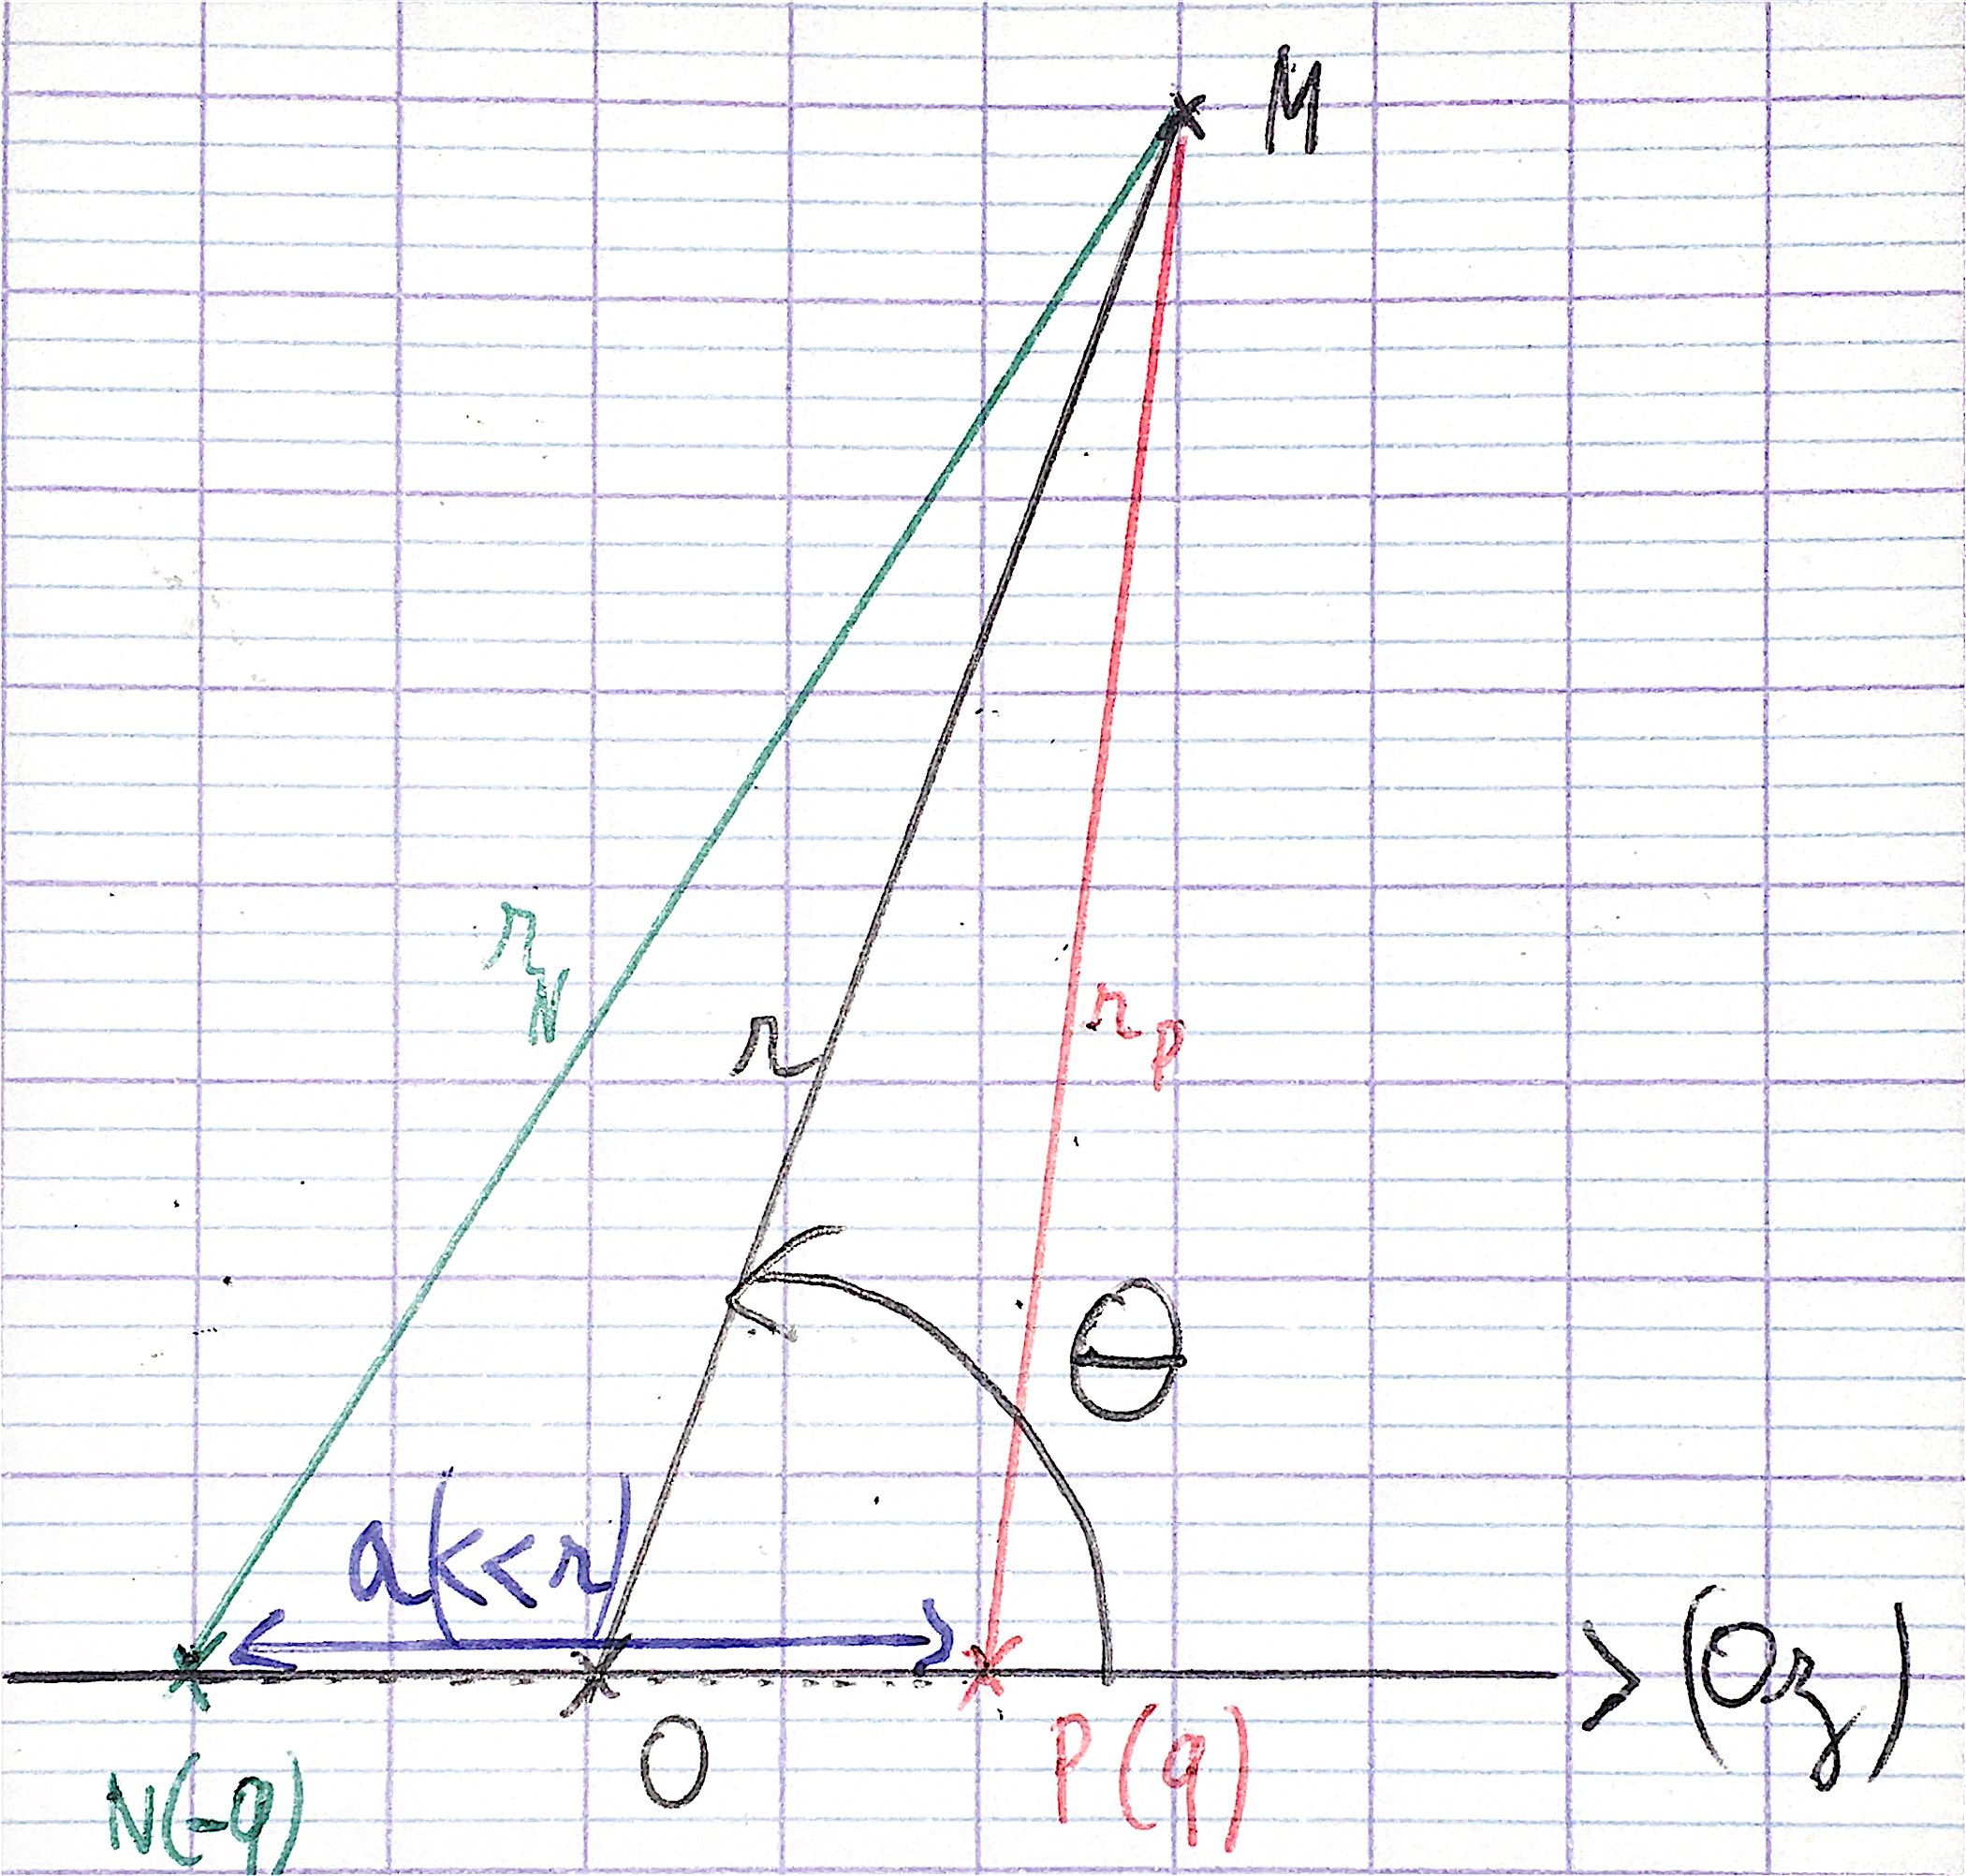
\includegraphics[height=15em]{dipole.jpg}
    \end{center}
    Une grandeur caractérisant un dipôle est son \notion{moment dipolaire $\vec{p}$}~:
    $$\vec {p} = q\vec{NP}$$
    Il s'exprime en $\mr{C}\cdot \mr{m}$.
\end{definition}

\end{adjustwidth}
\end{document}